\chapter{Implementation}
The approach taken in implementing this project was to break the system into two separate components. The first was the development of the vision algorithm in a Java SE environment on the desktop and the second was the development of the Android application.

The vision component was separated to create a simpler development environment, which enabled more rapid iteration due to the less constrained development environment. At the time it was expected to be relatively easy to port the Java wrapped OpenCV functions to the Android native environment, but this proved to be more difficult than initially planned. 

\section{Vision component}
From the beginning of this project it was understood that the vision component would be challenging to implement. In order to maximise success in this area it was decided to develop this component in the Java SE desktop environment as this offered ease of debugging and input of data from images stored on disk or live data taken from a web-cam. In addition developing in this manor was excellent for performing experiments and being able to capture the results in either image or plain text form.

\subsection{JavaCV}

This development stage utilised the JavaCV project which provides a Java interface to OpenCV through the Java Native Access library (JNA). Because the JavaCV wrapped functions match those exactly in the C-based library an excellent level of documentation is available online.

Using this JNA approach to call native functions from the managed environment incurs a performance penalty, JNA is up to 10X slower than its equivalent JNI call \cite{sun11}.  Although this maybe overcome using JNA direct mapping. 

This performance penalty was not of great concern, as the goal was to develop an object identification technique for a resource starved environment. Also maintaining the API level compatibility was vitally important for porting the techniques to the Android application.

\section{Android application}
The Maple Android application consisted of two components, the managed component and the native component which called the native OpenCV libraries. The managed component served mainly to call the native code and to layout the UI, while the native application handled all the image processing functionality.

\begin{figure}[h!]
\centering
    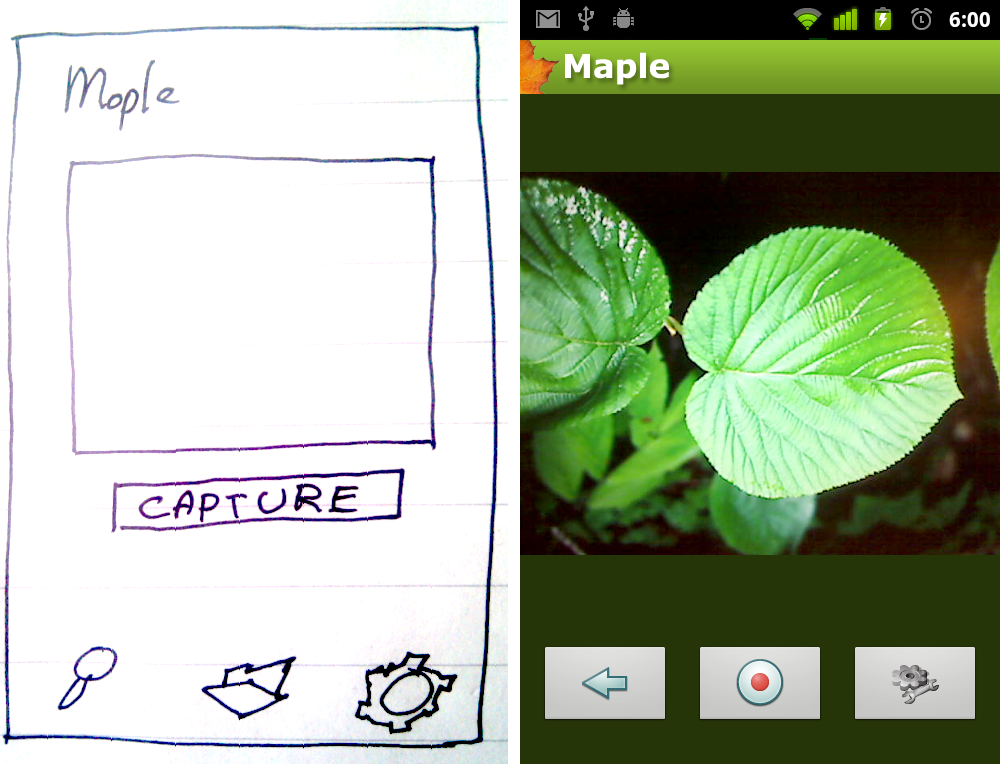
\includegraphics[width=0.8\textwidth]{implementation/images/mainscreen_mockup.png}
    \caption{Maple main interface UI: Early mockup (left), Implemented UI (right)}%
    \label{mainscreen_mockup}
\end{figure}

\subsection{Managed component}
The managed portion of the application consisted of an Activity class which determined the logic and the layout for the program and a number of Java JNI interface classes to provide an interface to the native component of the program.

We can see in Figure \ref{mainscreen_mockup} an early iteration of the concept for the UI (left) and the final implemented UI for the Application (right). The centre of the implemented UI provides feedback to the user by acting as a viewfinder. It was hoped that when complete the application would have no need for a record/capture button. The planned flow was when a leaf is identified the user would be automatically be shown an information page about the detected leaf. 

\subsection{Native component}
The native component for the project was by far the most difficult undertaking during the project. 

\begin{figure}[h!]
\centering
    \includegraphics[width=0.8\textwidth]{implementation/images/architecture_overview.pdf}
    \caption{Maple native architecture overview}%
    \label{native_architecture}
\end{figure}

\subsubsection{Structure}
In Figure \ref{native_architecture}, we see a high-level overview of the native call structure. The native image processing routine is called using Java Native Interfaces (JNI) for every frame captured from the camera by the managed code. This image is then stored in a native image pool and its index is passed to the native image processing routine.

The image processing routine gets a reference to the captured image using the image index passed in as a parameter. Processing is then performed on the image to identify objects of interest and any modifications that need to be made to the image is done at this stage. The image in the image pool is then updated with the modified image the the image processing routine returns.

Back in the managed application the native call which was placed in a callback list returns, invoking managed code to retrieve the image from the native image pool and update the image viewing portion of the view.

\subsubsection{Porting}
The porting of the object recognition code had proven to be more difficult than initially planned. This was due largely to the fact that only the OpenCV C++ library interface was available in the native environment, while the image processing functionality had been developed using Java wrappers of the C library interface.

OpenCV was originally written in C, but with the introduction of version 2.0 they introduced a C++ interface which utilised new data-structures for images, sequences and points. Because of this most of the function parameters had also changed. Also because the C++ interface is quite new online resources are not to the same standard as for the C-based interface.

This late discovery of the incompatibility was an oversight on behalf of the writer, and should have been investigated further during the research stage.

\subsubsection{File and data access}
When Android released the NDK with version 1.5 it was designed with the goal of performing single CPU bound functions that do not require much memory \cite{ndk11}. It was designed to avoid the writing of whole applications natively, as it is difficult to manage memory, life-cycle and resource locking correctly. For example allocating large quantities of memory in a native function can cause the whole device to perform poorly.

Because of this it is advised not to perform large parts of an applications functionality (with the exception of games) in the native environment and it is also not advised to access system resources natively.

It is possible however to read and write data to the filesystem, but this should be performed in another native class much like the image pool in Figure \ref{native_architecture} \cite{benfield10}. Performing read and write functions for every frame would be terribly inefficient. 

\subsubsection{Deployment}
Currently Android only targets two instruction sets (ARMv5TE and ARMv7-A) but there are plans to support a third in a future release (x86) \cite{ndk11}. This is not an issue for normal Android applications which are compiled for the Dalvik virtual machine, but for applications that include native code this may become a problem. Any native code that is deployed with the applications needs to be compiled for each of the architectures, letting Android pick at run-time the most appropriate.

When the OpenCV library is compiled for Android it requires 6.6 megabytes of space per instruction set. When the application is deployed to the phone the uncompressed size totals 13.3 megabytes.

This can become an issue on many current devices, even ignoring the fact that 13.3 megabytes is very large for mobile applications. When an application is downloaded from the Android Marketplace it requires twice the file-size of the application to be installed, so in our example to install this application the phone must have 26.6 megabytes of memory free. 

Further to this when you are deploying the application from the development environment it requires closer to three times the file-size in free memory to deploy the application. This is due to copying, extracting and installing with the application being already installed.

This problem can be overcome by reducing the size of the library to only the necessary functions. This however, was beyond the scope of the project.


